\capitulo{PROCEDIMENTOS METODOLÓGICOS E RESULTADOS}\label{sec:metodologia}
\iniciocapitulo

Este capítulo descreve os procedimentos metodológicos que foram necessários para a conclusão deste trabalho.

\secao{Análise do SMA desenvolvido pelo Grupo de Estudo de Engenharia de Software em Sistemas Multiagente (GESMA)}
\label{sec:analisesma}

O \textit{SMA Moodle} foi desenvolvido utilizando o \textit{framework JADE}, uma extensão denominada \textit{JAMDER} e respeitando os padrões do protocolo de comunicação \textit{FIPA}, que são tecnologias já descritas na Seção \ref{sec:multiagentes}.

O SMA interage com os dados do \textit{Moodle} através do acesso ao banco de dados deste AVA. Através da captura das informações do banco de dados, o SMA atualiza as informações acessíveis aos agentes. Os agentes podem postar mensagens em fóruns, utilizam \textit{chats}, criação de links ou arquivos no ambiente.

  Os agentes já em funcionamento no sistema são: agente companheiro de aprendizagem, agente pedagógico, agente acompanhante de tutores, agente fornecedor de materiais, agente formador de grupos e o agente auxiliar de usabilidade. Os agentes citados anteriormente serão descritos com mais detalhes logo a seguir, explorando suas principais características e responsabilidades de acordo com Gonçalves et al. (\citeyear{gonccalvesabordagem}):

\begin{enumerate}
\item \textbf{Agente Companheiro de Aprendizagem}: O Agente Companheiro de Aprendizagem é responsável por auxiliar o processo de aprendizagem dos alunos no decorrer do curso. De acordo com o desempenho do aluno, o agente envia mensagens para eles. Estas mensagens podem conter informações de apoio, reforço ou sugestões de atividades.
\item \textbf{Agente Pedagógico}: O Agente Pedagógico tem a responsabilidade de acompanhar e dar sugestões aos usuários em seus respectivos cursos, disciplinas e projetos.
\item \textbf{Agente Acompanhante de Tutores}: O Agente Acompanhante de Tutores é o agente responsável por acompanhar e monitorar os tutores em seus respectivos cursos dando sugestões sobre materiais de estudo antes das disciplinas começarem, como também dicas em relação a participação do mesmo em fóruns e na postagem de material didático.
\item \textbf{Agente Fornecedor de Materiais}: Este agente tem como principal característica enviar conteúdo digital de acordo com a disciplina especificada. Seu trabalho é realizado em conjunto com o Agente Companheiro de Aprendizagem. De acordo com o desempenho do aluno, caso o seu rendimento torne-se baixo ao decorrer do curso, este agente se responsabiliza de enviar material complementar por meio de postagens de arquivos ou \textit{link} no \textit{Moodle}, como também por meio de \textit{e-mails} e \textit{twitters}.
\item \textbf{Agente Formador de Grupos}: Este agente é responsável por criar grupos de usuários de acordo com características que indiquem afinidade, como perfis, temas e aprendizagem. Como o Agente Fornecedor de Materiais, ele também trabalha junto ao Agente Companheiro de Aprendizagem.
\item \textbf{Agente Auxiliar de Usabilidade}: O Agente Auxiliar de Usabilidade é responsável por auxiliar os novos usuários como também os veteranos em relação a possíveis dificuldades dos mesmos em relação ao AVA.
\end{enumerate}

Os agentes descritos correspondem ao corpo principal do SMA em questão. Sua execução acontece em conjunto ao \textit{Moodle} e os seus dados são alimentados de acordo com os dados contidos na base de dados do AVA.

\secao{Análise da Base de Dados do Moodle da Universidade Estadual do Ceará (UECE) e Seleção de Algoritmos para Mineração}
\label{sec:analise}

O AVA \textit{Moodle} é um sistema modular, que possui o gerenciamento de vários módulos voltados ao gerenciamento dos cursos. A sua estrutura relacional do banco de dados reflete essa característica.

\subsecao{Análise}

As tabelas no banco de dados são compostas pelo prefixo e nome do módulo. O prefixo padrão é o \textit{mdl\_}. Isso pode ser alterado no momento da instalação. Por exemplo, a tabela do módulo Curso é mdl\_course. Todos os módulos seguem esse padrão.

Cada módulo possui uma tabela principal e tabelas secundárias. A estrutura da nomenclatura dessas tabelas são:
\begin{enumerate}
\item Tabela Principal: \textit{mdl\_} + nome do modulo. Ex: mdl\_course.
\item Tabela Secundaria: \textit{mdl\_} + nome do modulo + funcionalidade do módulo. Ex: mdl\_course\_categories.
\end{enumerate}

Vale ressaltar que alguns conceitos das nomenclaturas dos componentes do \textit{Moodle} diferem dos utilizados comumente nas Instituições de Ensino. Um exemplo comum é sobre o módulo de cursos. Na verdade cursos para o \textit{Moodle} são disciplinas para uma Universidade, por sua vez, esse conjunto de cursos fazem parte de um grupo, que correspondem a matriz curricular de disciplinas que compõem um curso para a Instituição de Ensino.

Para o presente trabalho, os módulos mais importantes foram:
\begin{enumerate}
\item \textbf{\textit{User}}: para a captura dos alunos matriculados na plataforma.
\item \textbf{\textit{Course}}: para obter os cursos registrados no banco de dados e em quais cursos cada aluno esta matriculado.
\item \textbf{\textit{Log}}: para capturar os dados de participação do aluno
\item \textbf{\textit{Grades}}: para obter as notas das avaliações dos alunos.
\end{enumerate}

\subsecao{Seleção}

Os dados fornecidos para o presente trabalho correspondem a uma quantidade de 3195 alunos, 248 cursos e de um intervalo de tempo de Agosto de 2011 à Agosto de 2013.

No presente trabalho de acordo a analise do banco de dados e estudos dos trabalhos relacionados, foi possível selecionar as informações mais importantes que correspondessem às interações dos usuários na plataforma para a construção do modelo de dados em questão. Elas foram escolhidas por serem os valores quantitativos que mais são utilizados pelos alunos. As informações elencadas no processo de Seleção dos Dados foram:

\begin{enumerate}
\item Identificação do Aluno
\item Identificação do Curso
\item Data de Criação do Curso
\item Data que o Curso Iniciará
\item Média Final de Cada Curso
\item Período Semanal
\item Período Mensal
\item Período Semestral
\item Quantidade de Acessos ao Curso
\item Quantidade de Acessos ao Fórum
\item Quantidade de Postagens no Fórum
\item Quantidade de Atividades Entregues
\item Média das Notas das Atividades
\item Quantidade de Acessos aos Arquivos
\item Quantidade de Acessos às Wikis
\end{enumerate}

\subsecao{Pré-Processamento}

Para a construção do modelo, foram utilizados atributos que passaram por pré-processamento para que fossem obtidos, visto que as informações contidas neles não estavam de forma clara (como o modelo precisava) e organizadas no banco de dados do \textit{Moodle}. Para isso foi criado um \textit{Data Mart} que será alimentado mensalmente, e que também servirá para guardar o histórico de acompanhamento dos alunos ao decorrer do período acadêmico.

Para a etapa de pré-processamento, foi desenvolvida uma aplicação na linguagem \textit{Java}\footnote{Disponível em: https://www.java.com/pt\_BR} utilizando \textit{JDBC}\footnote{Disponível em: http://www.oracle.com/technetwork/java/javase/jdbc/index.html} no ambiente de desenvolvimento \textit{Eclipse}\footnote{Disponível em: https://eclipse.org}. Essa aplicação mapeia o banco de dados do \textit{Moodle} tendo como finalidade capturar as informações necessárias para alimentar o \textit{Data Mart}.

\subsecao{Organização e Alimentação do \textit{Data Mart}}

O \textit{Data Mart} é composto por um conjunto de tabelas que suprem às informações necessárias para a construção e atualização do modelo de dados do presente trabalho, como também para o gerenciamento do acompanhamento semestral dos alunos que é realizado pelo modulo de evasão desenvolvido nesse trabalho. Inicialmente ele foi alimentado com os dados históricos dos alunos contidos no intervalo de Agosto de 2011 a Agosto de 2013, para que um modelo de dados inicial fosse definido. Os dados foram obtidos de todos os cursos registrados no banco de dados que tiveram registros dos atributos destacadas na etapa de seleção. A seguir será descrito sucintamente cada uma das tabelas e suas finalidades.

\begin{enumerate}
\item \textbf{\textit{Semester}}: tabela que é registrado cada semestre letivo, para que tenha o controle da captura das informações correspondentes a cada semestre.
\item \textbf{\textit{Course}}: a cada semestre é registrado os cursos ofertados para os alunos.
\item \textbf{\textit{Week Control}}: é dividido para cada curso um agrupamento de dados em janelas de tempo para que os dados de participação de cada aluno seja capturado. Aproximadamente são divididos em 19 semanas que correspondem a um semestre letivo.
\item \textbf{\textit{Month Control}}: para cada curso é registrado um período mensal para que aconteça a classificação do status daquele aluno. Por \textit{default} é configurado para registrar bimestralmente ou conforme seja configurado pelo administrador do sistema.
\item \textbf{\textit{Student e Student Course}}: a tabela \textit{Student} é utilizada para salvar todos os alunos matriculados do \textit{Moodle} e referencia-los com seus respectivos cursos com a tabela \textit{Student Course}.
\item \textbf{Historic}: é a tabela mais importante, onde serão registrados os dados semanalmente de cada aluno em relação aos cursos matriculados naquele semestre. O atributo \textit{register\_type} corresponde ao tipo de registro que está sendo armazenado. Os tipos de registro são:
\begin{itemize}
\item QAC: Quantidade de Acessos ao Curso
\item QAF: Quantidade de Acessos ao Fórum
\item QPF: Quantidade de Postagens no Fórum
\item QAA: Quantidade de Acessos aos Arquivos
\item QAW: Quantidade de Acessos às Wikis
\item QAE: Quantidade de Atividades Entregues
\item MNA: Média das Notas das Atividades
\end{itemize}
\item \textbf{\textit{Accompaniment}}: esta tabela será alimentada com a verificação bimestral dos alunos pelo processo de classificação, que será explicado na próxima subseção. O atributo \textit{status} corresponde aos grupos em que os alunos são divididos em relação aos seus dados quantitativos, os valores que esse atributo pode assumir são:
\begin{itemize}
\item MUITO BAIXO RISCO
\item BAIXO RISCO
\item REGULAR
\item RISCO
\item FORTE RISCO
\end{itemize}
\end{enumerate}

A figura \ref{fig:modelodatawarehouse} ilustra o modelo Entidade Relacionamento da entidades que contemplam o \textit{Data Mart}.

\begin{figure}[!ht]
\caption{Modelo Entidade Relacionamento do \textit{Data Mart}}
\centering
\fbox{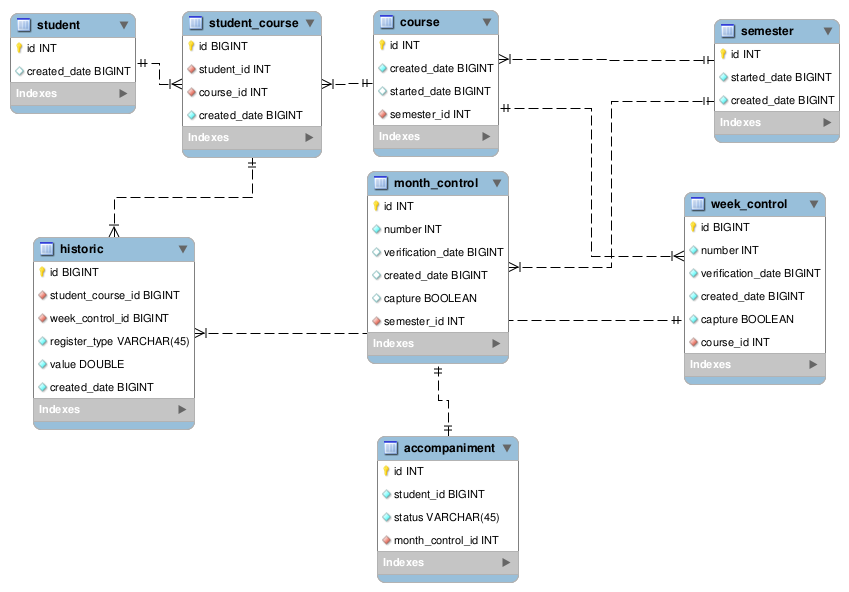
\includegraphics[width=0.75\textwidth]{imagens/model_data_warehouse.png}}
\caption*{Fonte: fornecido pelo autor}
\label{fig:modelodatawarehouse}
\end{figure}

\secao{Análise comparativa para a escolha de uma Ferramenta que auxilie o processo de Extração de Conhecimento}

Foi realizado uma analise comparativa entre três ferramentes que podem auxiliar no processo de KDD. As ferramentas são:
\begin{enumerate}
\item RapidMiner
\item Weka
\item Elki
\end{enumerate}

Para a escolha da ferramenta ideal foram definidas alguma métricas, das quais a que foi mais relevante foi, se a ferramente possui \textit{API} para ser utilizados seus métodos de descoberta de conhecimento em \textit{Java}, pelo fato do modulo desenvolvido no presente trabalho ser nessa linguagem, visto que os agentes que serão explicados na Seção seguinte, encapsulam todo o processo de KDD.

Além de analisar se as ferramentas possuíam \textit{API}, foram verificados a popularidade e documentação das mesmas. O gráfico \ref{fig:comparativoferramentas} da popularidade das ferramentas aqui citadas.

\begin{figure}[!ht]
\caption{Comparativo da Popularidade das Ferramentas}
\centering
\fbox{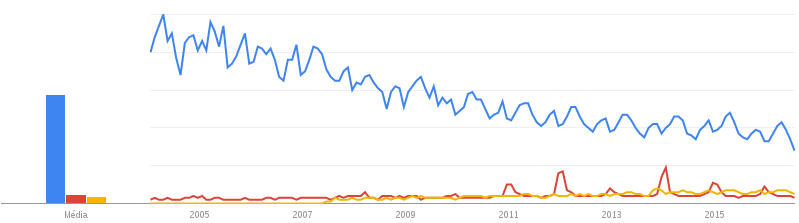
\includegraphics[width=0.75\textwidth]{imagens/comparativo_ferramentas.png}}
\caption*{Fonte: Gerado no Google Trends}
\label{fig:comparativoferramentas}
\end{figure}

No gráfico \ref{fig:comparativoferramentas} a cor azul representa a popularidade da ferramenta \textit{Weka}, a cor vermelha representa a popularidade da ferramenta \textit{Elki}, e por sua vez, a cor amarela representa a popularidade da ferramenta \textit{RapidMiner}, diferente das outras ferramentas já citadas, o \textit{RapidMiner} não é \textit{open source}. Os dados foram comparados com informações obtidas de 2005 a 2015, em relação as buscas relacionadas às ferramentas no buscador do \textit{Google}\footnote{Disponível em: http://google.com}.

A ferramenta escolhida foi a \textit{Weka}, por conter uma boa documentação e interface agradável de manipulação, proporcionando assim uma curva mínima de aprendizagem.

\subsecao{Modelo, Mineração dos Dados e Descoberta de Padrões}
\label{sec:modelo}

Para a construção do Modelo foi utilizada a \textit{API} fornecida pela ferramenta \textit{Weka}. Através dela foi possível utilizar na linguagem \textit{Java} os métodos necessários os passos a seguir. Após o \textit{Data Mart} ser alimentado com os dados históricos dos alunos que já estão cursaram, os dados são agrupados por aluno em um arquivo \textit{arff}, essa escolha é derivada da eficiência que é obtida utilizando ele em conjunto com a \textit{API} do \textit{Weka}, visto que tipo de arquivo foi desenvolvido especificamente para ser usado pela ferramenta. Cada instancia do modelo de dados é composta pelos seguintes atributos:

\begin{table}[!ht]
\centering
\caption{Descrição dos Dados que compõem o Modelo Inicial}
\vspace{0.5cm}
\begin{tabular}{l|r|r|}
 
Atributo & Descrição & Tipo\\
\hline
QAC & Quantidade de Acessos ao Curso& Numérico\\
QAF & Quantidade de Acessos ao Fórum& Numérico\\
QPF & Quantidade de Postagens no Fórum& Numérico\\
QAE & Quantidade de Atividades Entregues& Numérico\\
MNA & Média das Notas das Atividades& Numérico\\
QAA & Quantidade de Acessos aos Arquivos& Numérico\\
QAW & Quantidade de Acessos às Wikis& Numérico
\end{tabular}
\label{tab:modelo_inicial}
\end{table}

Para que fosse possível dividir os alunos em grupos de acordo com seus dados quantitativos capturados ao decorrer do tempo, foi utilizado um algoritmo aprendizagem não supervisionada, o \textit{K-Means}, a escolha desse algoritmo para esse contexto foi influenciada pelo trabalho de  Silva, Machado e Araújo (\citeyear{silva2014sistema}), que se assemelha com o problema abordado nesse trabalho. O \textit{K-Means} é um algoritmo de clusterização, já explicado na Seção \ref{sec:silva}. Após o processo de clusterização no modelo de treinamento, os dados foram divididos em 5 grupos (MUITO BAIXO RISCO, BAIXO RISCO, REGULAR, RISCO e FORTE RISCO). O fator determinante para que os grupos fossem divididos da seguinte forma, foi o atributo de média das notas das avaliações realizadas (MNA). Cada grupo ficou dividido da seguinte forma:

\begin{enumerate}
\item MUITO BAIXO RISCO: 9\% dos dados equivalente a 298 alunos.
\item BAIXO RISCO: 19\% dos dados equivalente a 618 alunos.
\item REGULAR: 20\% dos dados equivalente a 641 alunos.
\item RISCO: 15\% dos dados equivalente a 472 alunos.
\item FORTE RISCO: 36\% dos dados equivalente a 1166 alunos.
\end{enumerate}

De acordo com os atributos utilizados para a construção do modelo clusterizado, a tabela a seguir demonstra os valores iniciais de cada atributo que determina a entrada da instancia no \textit{cluster} correspondente, que é encontrado após executar o algoritmo \textit{K-Means} no \textit{dataset} atual. Foi utilizada a técnica distância euclidiana como método do calculo de similaridade, que é uma técnica que mede a distancia entre dois pontos, essa escolha não teve nenhum motivo especifico, pois não foi testado outras técnicas para calcular a similaridade e comparar os resultados, a técnica Distância Euclidiana é configurada por \textit{default} no \textit{Weka}. Vale ressaltar, que esses valores podem mudar ao longo do tempo, conforme novos dados vão sendo inseridos no \textit{data mart}. A figura \ref{fig:arff} ilsutra uma pequena parte do arquivo \textit{arff} gerado e o gráfico \ref{fig:variancia} ilustra a variância de cada atributo em relação aos seus valores.

\begin{figure}[!ht]
\caption{Visualização de uma pequena parte do Arquivo \textit{Arff} gerado após a etapa de clusterização}
\centering
\fbox{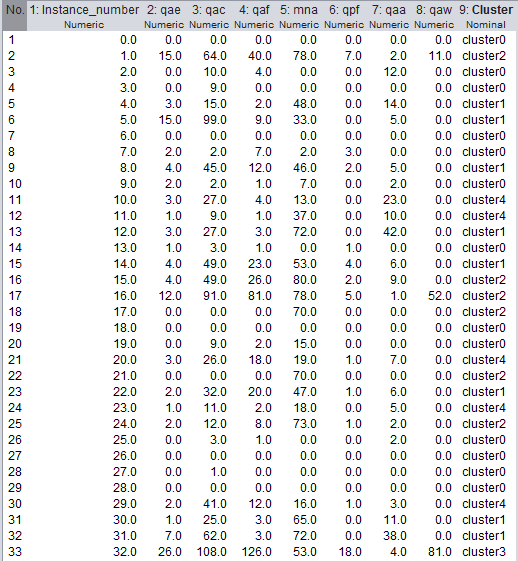
\includegraphics[width=0.72\textwidth]{imagens/arff.png}}
\caption*{Autor: Fornecido pelo Autor}
\label{fig:arff}
\end{figure}

\begin{table}[!ht]
\centering
\caption{Valores iniciais que determinam em qual \textit{cluster} cada instancia corresponde}
\vspace{0.5cm}
\begin{tabular}{l|r|r|r|r|r|r|r|} 
Cluster & QAE & QAC & QAF & MNA & QPF & QAA & QAW\\
\hline
MUITO BAIXO RISCO & 30 & 307 & 299 & 92 & 101 & 28 & 86\\
BAIXO RISCO & 9 & 148 & 82 & 86 & 9 & 6 & 21\\
REGULAR & 3 & 65 & 14 & 77 & 0 & 21 & 0\\
RISCO & 1 & 8 & 3 & 19 & 0 & 3 & 0\\
FORTE RISCO & 0 & 0 & 0 & 0 & 0 & 0 & 0\\
\end{tabular}
\label{tab:modelo_clusterizado_valores}
\end{table}

\begin{figure}[!ht]
\caption{Mapa de calor dos \textit{clusters}, onde cada cor representa um \textit{cluster} em ordem crescente}
\centering
\fbox{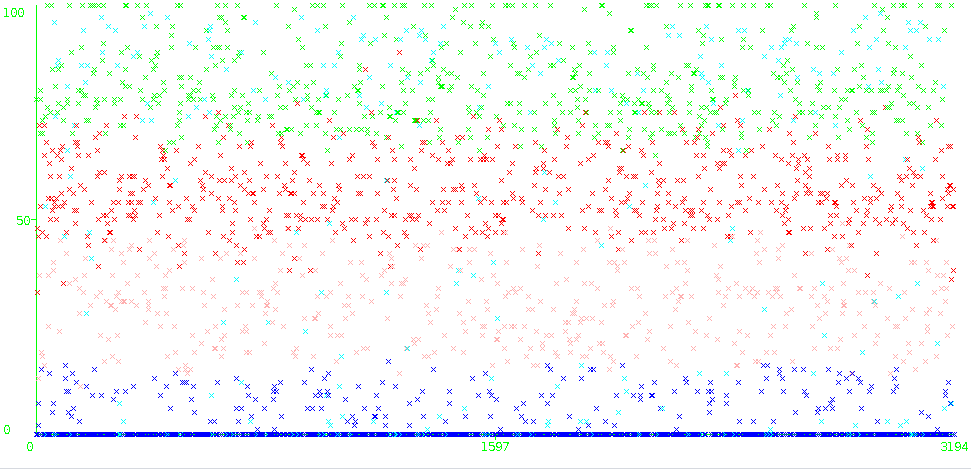
\includegraphics[width=0.72\textwidth]{imagens/mapa_calor.png}}
\caption*{Autor: Fornecido pelo Autor}
\label{fig:mapa_calor}
\end{figure}

\begin{figure}[!ht]
\caption{Gráfico de variância dos valores dos atributos}
\centering
\fbox{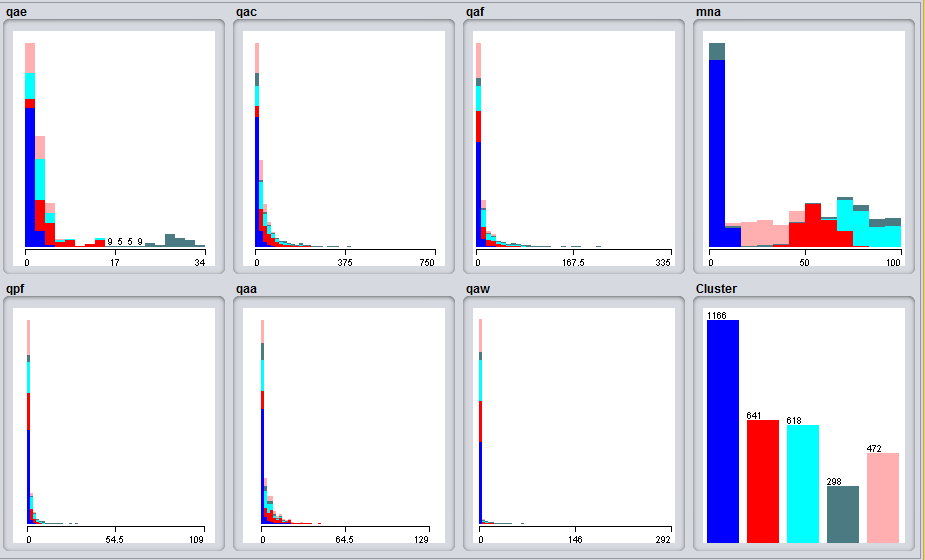
\includegraphics[width=0.72\textwidth]{imagens/atributos.png}}
\caption*{Autor: Fornecido pelo Autor}
\label{fig:variancia}
\end{figure}

Na figura \ref{fig:mapa_calor} o eixo $X$ representa a quantidade de alunos, o eixo $Y$ representa a faixa de valores do atributo \textit{MNA}. A cor azul escura representa o \textit{cluster} FORTE RISCO, a rosa o RISCO, o vermelho o REGULAR, o verde o BAIXO RISCO e o azul claro o MUITO BAIXO RISCO. 

Os alunos que foram alocados aos grupos RISCO e FORTE RISCO, são alunos que possuem mal desempenho em suas interações com a plataforma, sendo fortes concorrentes a desistirem do curso. Os alunos que são classificados com esses \textit{status} são os que sofrem intervenção do SMA para melhorarem seu desempenho educacional.

Com a descoberta das classes foi realizado um teste comparativo entre cinco algoritmos e avaliado o que teve a maior acurácia em relação aos dados do modelo. Os algoritmos testados foram: \textit{SimpleCart}, \textit{J48}, \textit{JRip} (equivalente ao RuleLearner) e \textit{Random Forest}.

A tabela a seguir apresenta a acurácia de cada algoritmo em relação ao modelo de dados. Para a verificação foi utilizada a técnica \textit{cross-validation}, já explicada na Seção \ref{sec:mineracao}. Os dados foram divididos em 10 \textit{folds}.

\begin{table}[!ht]
\centering
\caption{Comparação entre os algoritmos de Classificação em relação a Acurácia}
\vspace{0.5cm}
\begin{tabular}{l|r|r|}
 
Algoritmo & Acurácia\\
\hline
\textbf{\textit{SimpleCart}} & 97,24\%\\
\textbf{\textit{J48}} & 97,32\%\\
\textbf{\textit{JRip}} & 96,95\%\\
\textbf{\textit{Random Forest}} & 98,27\%
\end{tabular}
\label{tab:comparacao_algoritmos}
\end{table}

Através da comparação de acurácia dos algoritmos em relação ao modelo de treinamento, o \textit{Random Forest} foi o que obteve o melhor resultado, sendo assim o escolhido para ser utilizado no módulo desenvolvido no presente trabalho. A acurácia dos algoritmos foi determinada de acordo com a Métrica de \textit{Kappa}, que é uma forma de medir a concordância das interpretações dos valores de cada instancia do modelo.

\subsection{Atualização do Modelo}

Ao final de cada semestre letivo, os dados históricos capturados dos alunos serão integrados com os dados históricos utilizados para a definição do modelo de dados inicial. Após isso, o modelo passará novamente pelo processo de clusterização, para que as classes sejam atualizadas e o modelo para predição fique cada vez mais inteligente acompanhando os padrões de interação dos alunos com a plataforma.

\secao{Desenvolvimento da Arquitetura do Módulo de Evasão do SMA do GESMA}

Para o presente trabalho foi possível identificar alguns papéis que o módulo em questão deve suprir. Esses papéis são:
\begin{enumerate}
\item Controlar o Tempo em que um Semestre Inicia e Termina, para capturar os dados e alimentar o \textit{Data Mart} periodicamente.
\item Capturar os Dados periodicamente das interações dos alunos no \textit{Moodle}.
\item Classificar os alunos bimestralmente.
\item Comunicar os demais agentes do ambiente sobre o que foi interpretado com a classificação dos alunos, para que os demais agentes tomem decisões para auxiliar o aluno a melhorar o desempenho e terem êxito nos cursos matriculados.
\end{enumerate}

Para que fosse possível atender esses papéis foi desenvolvido o Agente Controlador de Evasão. Este Agente possui encapsulado em seus comportamentos todo o processo de KDD descrito na Seção \ref{sec:analise}, como também a comunicação com os demais agentes do SMA, principalmente com o Agente Companheiro de Aprendizagem, cujo suas características já foram descritas na Seção \ref{sec:analisesma}.

O fluxo dos processos executados pelos comportamentos do Agente Controlador de Evasão será descrito a seguir:

\begin{enumerate}
\item Verificação se a data atual de execução está dentro do intervalo de tempo correspondente ao semestre atualmente cadastrado.
\item Caso a data não esteja entre o intervalo de tempo correspondente ao semestre atualmente cadastrado, o comportamento do Agente Controlador de Evasão se encerra nesse ciclo.
\item Caso a data atual esteja dentro do intervalo de tempo, ele irá verificar os cursos que foram registrados para serem ofertados durante aquele semestre letivo.
\item Com a identificação dos Cursos, ele irá registrar no \textit{Data Mart} o período semanal que deverá ocorrer a captura dos dados.
\item Analogamente ao período semanal, ele irá registrar o período mensal em que deverá acontecer a classificação dos alunos para obter a cada etapa o estado do desempenho do aluno.
\item Se a data atual corresponder a algum dia que deverá ocorrer a captura dos dados, o Agente irá capturar os dados de cada aluno por curso, em um intervalo de uma semana. Os dados capturados semanalmente já foram descrito conforme na Seção \ref{sec:modelo}.
\item Se a data atual corresponder a algum dia que deverá ocorrer a classificação dos dados dos alunos, o Agente irá agrupar os dados capturados do inicio do semestre até aquela data, e irá classificar o aluno utilizando o algoritmo \textit{Random Forest} que estará encapsulado dentro do seu comportamento através da \textit{API} do \textit{Weka}. O modelo que servirá como base para classificar o \textit{status} desse aluno, é o modelo construído após o processo de clusterização.
\item Identificando os alunos que possuem o \textit{status} referente aos grupos de alunos RISCO e FORTE RISCO, serão encaminhados para o Agente Companheiro de Aprendizagem, para que ele se responsabilize em auxiliar esses alunos a mudarem esse cenário de mau desempenho que tendem a evasão do curso e enviará por e-mail a relação de alunos com essa classificação para os professores/tutores e coordenadores.
\item Por fim, ao chegar no final do semestre corrente, o Agente irá agrupar todos os dados históricos de todos os alunos até o momento, executar o processo de clusterização para dividir os alunos nos grupos definidos na Seção \ref{sec:modelo}, assim atualizando o modelo de predição de dados.
\end{enumerate}

Após a definição dos papéis e de como se comunicar com os Agentes necessários, foi iniciada a etapa de implementação do Agente Controlador de Evasão.

\secao{Implementação do Sistema}

O Agente Controlador de Evasão foi desenvolvido utilizando o \textit{framework JADE} com a extensão \textit{JAMDER}, de acordo com as definições descritas na subseção anterior.
No Agente foi definido um comportamento cíclico, que é executado uma vez por dia. Nele estão todos os passos de execução descritos na subseção anterior.

A interação do Agente Controlador de Evasão com o banco de dados do \textit{Moodle} e com o \textit{Data Mart} foi desenvolvida utilizando \textit{JDBC} com o banco de dados \textit{PostgreSQL}\footnote{Disponível em: https://www.postgresql.org/}. Para as interações do Agente Controlador de Evasão com o banco de dados do \textit{Moodle}, foram aproveitados os métodos já implementados no SMA. A interface de interação entre o SMA e o banco de dados do \textit{Moodle} foi desenvolvida utilizando o \textit{framework Hibernate} \footnote{Disponível em: http://hibernate.org/}, que é um \textit{framework} que realiza o mapeamento objeto relacional \textit{Object Relational Mapper} (ORM), tendo como finalidade diminuir a complexidade do desenvolvimento da persistência dos dados.

\secao{Execução, Coleta de Dados e Testes}

Para esta etapa o Agente Controlador de Evasão foi executado em um ambiente separado do SMA simulando um ambiente real de atividade, a fim de observar seu comportamento em relação a gerencia do processo de KDD nele encapsulado. Como já descrito na Seção \ref{sec:modelo}, foram utilizados para testes os dados de 3195 alunos, 248 cursos e de um intervalo de tempo de Agosto de 2011 à Agosto de 2013. Após o Agente alimentar o \textit{Data Mart} com as informações necessárias para construir o modelo de treinamento, o modelo foi submetido a um processo de clusterização, como já descrito na Seção \ref{sec:modelo}, utilizando o algoritmo \textit{K-means}, a fim de descobrir as classes necessárias para a predição. Após a descoberta dos grupos, o modelo foi submetido ao processo de {cross-validation} com o algoritmo \textit{Random Forest}, validando a predição obtendo uma acurácia de 98,27\%.

\secao{Análise e Validação dos Resultados Obtidos}

 Com o \textit{Data Mart} alimentado pelo Agente, a predição foi testada e validada de duas formas:

\begin{enumerate}
\item Através da Técnica de \textit{Cross-validation}, já descrita na Seção \ref{sec:mineracao}, no qual com o algoritmo \textit{Random Forest} foi obtido uma acurácia de 98,27\%.
\item Foi fornecido pela UECE uma planilha contendo a relação de alunos divididos entre alunos graduados, desistentes, que abandonaram e que foram transferidos do curso.
\end{enumerate}

A planilha continha a relação de alunos já matriculados no período de 2006 a 2014 nos cursos ofertados pela UAB/UECE, totalizando 3359 alunos, dos quais 405 são alunos desistentes. Apesar da planilha ser de um espaço de tempo maior do que o dos dados encontrados no \textit{Moodle}, foi possível identificar em 92.5\% dos alunos que poderiam evadir resultantes da predição em comparação com os alunos desistentes apontados na planilha.

Através dessas informações reais dos alunos, houve uma comparação com o histórico de predição. Houve casos em que alunos considerados bons pela etapa de classificação foram identificados como alunos desistentes ou que abandonaram o curso, esse tipo de caso é impossível prever, pois provavelmente partiu de uma causa externa em relação ao aluno e sua vida pessoal. Em contra partida todos os alunos que tiveram como causas de suas desistências apenas problemas em relação com a plataforma, foi possível prever com a técnica de classificação.